\ProvidesFile{rutitlepage.dtx}[2022/02/21 v3.0 Radboud University Titlepage]
\documentclass{ltxdoc}
\newcommand{\messagespace}{\text{$\mathcal{M}$}}
\newcommand{\messageinstance}{\text{$m$}}
\newcommand{\ciphertextspace}{\text{$\mathcal{C}$}}
\newcommand{\ciphertextinstance}{\text{$c$}}
\newcommand{\associateddataspace}{\text{$\mathcal{A}$}}
\newcommand{\associateddatainstance}{\text{$a$}}
\newcommand{\tagspace}{\text{$\mathcal{T}$}}
\newcommand{\taginstance}{\text{$t$}}
\newcommand{\keyspace}{\text{$\mathcal{K}$}}
\newcommand{\keyinstance}{\text{$k$}}
\newcommand{\noncespace}{\text{$\mathcal{N}$}}
\newcommand{\nonceinstance}{\text{$n$}}
\newcommand{\lockspace}{\text{$\mathcal{L}$}}
\newcommand{\lockinstance}{\text{$l$}}
\newcommand{\users}{\text{$N$}}
\newcommand{\user}{\text{$j$}}
\newcommand{\adversary}{\text{$A$}}
\newcommand{\sample}{\text{$\leftarrow$}}
\newcommand{\result}{\text{$\leftarrow$}}
\newcommand{\concatinate}{\text{$\|$}}

\newcommand{\advantage}[2]{\textbf{Adv}$_{\text{#1}}^{\text{#2}}$ }
\newcommand{\probabilityblock}[4]{\text{$|\text{Pr}[\text{#1}_{\text{#2}}^{\text{#3}}] - \text{Pr}[\text{#1}_{\text{#2}}^{\text{#4}}]|$}}

\newcommand{\pkc}{\text{Hybrid Encryption in a Multi-user Setting, revised}}
\newcommand{\gcrec}{\text{Generic Composition Reconsidered}}

\newcommand{\x}{\text{x}}
\usepackage{a4wide}
\usepackage{float}
\usepackage{graphicx}
\usepackage{array}
\usepackage[utf8]{inputenc}
\usepackage{rutitlepage}
\usepackage{fancyhdr}
\usepackage[style=ieee]{biblatex}
\usepackage[operators]{cryptocode}
\usepackage{amssymb}
\addbibresource{cryptobib/crypto.bib}
\GetFileInfo{rutitlepage.dtx}
\newtheorem{theorem}{Theorem}

\pagestyle{fancy}
\fancyhf{}
\lhead{Bachelor Thesis}
\rhead{Page \thepage}

\title{Bachelor Thesis Stijn Vandenput}
\author{stijnvandenput }
\date{20 May 2022}

\begin{document}
\maketitleru[
    layout=traditional,
    authors={Stijn Vandenput},
    authorstext={Author:},
    nextpagenr={-1},
    date={20/05/2022},
    institution={Radboud University},
    others={Supervisors:}{Martijn Stam\\Bart Mennink},
    course={Bachelor Thesis},
    title={TBD}]

\section*{Abstract}

\pagenumbering{roman}
\newpage
\tableofcontents

\newpage
\pagenumbering{arabic}

\section{Introduction}
Although symmetric and asymmetric cryptography are both subfields of cryptography, their research area's can be quite separated. This can lead to knowledge gaps between the two whenever work in asymmetric crypto uses constructions that are more common in symmetric crypto or the other way around. In this fashion, a paper by Giacon, Kiltz and Poettering \cite{PKC:GiaKilPoe18}, which we henceforth call \gkp{}, uses a construction that is very similar to Authenticated Encryption following the generic encrypt-then-MAC construction from Bellare and Namprempre \cite{AC:BelNam00}. This construction has since been revised in a paper by Namprempre, Rogaway and Thomas Shrimpton \cite{EC:NamRogShr14}, which we henceforth call \nrs{}. In this revision, a new set of constructions is given that be better applicable to common use cases. The aim of this thesis is to apply the knowledge from \nrs{} to the setting of \gkp{} and, while doing so, create a new primitive for authenticated encryption suited for asymmetric settings.

\section{Preliminaries}
In this section we will explain several concepts important to the rest of our work, as well as some general notation.

\subsection{General Notation}
Strings are binary and bit-wise, the set of all strings is $\{0,1\}^\ast$. The length of $x$ is written as $\abs{x}$, the concatenation of $x$ and $y$ as $x$ \concatinate{} $y$, $a$ being the result of $b$ as $a$ \result{} $b$ and taking a random sampling from $y$ and assigning it to $x$ as $x$ \sample{} $y$. We write \users{} for the number of users and allow a single type of error message written as \invalid. We assume the existence of a nonempty key space \keyspace{}, a lock space \lockspace{}, a nonce space \noncespace{}, a message space \messagespace{} and a associated-data space \associateddataspace{}. Unless stated otherwise, \messagespace{} contain at least two strings, and if \messagespace{} or \associateddataspace{} contain a string of length $x$, it must contain all strings of length $x$.

\subsection{Authenticated Encryption}
Two different security requirements are data privacy, the insurance that data cannot be viewed by a unauthorized party, and data integrity, the insurance that data has not been modified by a unauthorized party. Authenticated encryption combines both of these security requirements into one and ensures both data privacy and integrity. In addition some authenticated encryption schemes allow you to provide additional data, AD. This data is specifically required to not have data privacy but does require data integrity. Authenticated encryption schemes that support AD are called AEAD schemes.

\subsection{Nonces and Locks improved}
Both nonces and locks are given as input to an encryption scheme. They prevent a message from leading to the same ciphertext when encrypted multiple times under the same key. Although they look similar, their purpose and exact working differ leading to different use cases.

\paragraph{Nonces}
Normally, when a message is encrypted twice by the same user, it results in the same ciphertext. This can leak information about the message, which can be prevented using a nonce. A nonce is a number that is assumed to only be used once per user to encrypt a message. Whenever a message is encrypted twice with the same key, but with two different nonces, the resulting ciphertexts should be indistinguishable from two ciphertexts corresponding to two different messages. As a result, it is infeasible for an adversary to guess if a message has been send multiple times. The adversary is usually allowed to let a user decrypt multiple messages with one nonce. Nonces are only used when a user uses its key multiple times, as otherwise a message will never be encrypted by the same user twice.

\paragraph{Locks}
Normally, when two users that have a key collision encrypt the same message, results in the the same ciphertext. This can leak information about the secret keys used, which can be prevented using locks. Whereas nonces are bound to the message, locks are bound to the user. Each user has one lock and will encrypt all their messages using that lock. (\textbf{Question: Locks are not exclusive to a one-time use key right?}) Whenever a message is encrypted twice with the same key, but with two different locks, the resulting ciphertexts should be indistinguishable from two ciphertexts corresponding to two different messages. As a result, it is infeasible for a adversary to see if two users have a key collision unless locks collide as well. To prevent this we assume locks to be globally unique. The adversary is usually only allowed to let a user decrypt messages with the correct lock. Locks are only used in a multi-user setting, as key collision is impossible when there is one user.  

\subsection{Security Notions}
The security of a cryptographic construction can be modeled as a distinguishing advantage. There are different things we can distinguish on, leading to different security notions. The relevant ones are written below.

\paragraph{IND-CPA vs IND-CCA}
You can model against an passive or an active attacker. A passive attacker can only read the messages while a active attacker can also alter the messages. A passive attacker can be modelled using a chosen plaintext attack, CPA for short. In this model, the adversary can choose the plaintext that is encrypted, but not the ciphertext that is decrypted. A active attacker can be modelled using a chosen ciphertext attack, CCA for short. In this model, the adversary can choose the plaintext that is encrypted, as well as the ciphertext that is decrypted. Shorthand notations for the two is IND-CPA and IND-CCA respectively. IND-CCA implies IND-CPA, but not the other way around.

\paragraph{IND-\$ vs IND-LOR}
Left or right indistinguishablility refers to a situation where the adversary gives two messages, and is given a ciphertext. The adversary has to guess which of the two messages corresponds to the ciphertext. \$ indistinguishablility refers to a situation where the adversary is given access to either the real construction, or to a random function \$. This random function returns a random string with the same length as the ciphertext would have. The adversary has to guess which of these two it has access to. As long as the length of the ciphertext is not randomized, IND-\$ implies IND-LOR, but not the other way around. (\textbf{todo: add citation})

\noindent\\
Both of these are separate dimension and can be combined into 4 different notations. For example IND-\$-CCA refers to a situation where the adversary has to distinguish between the real construction, or a random function while being able to choose both the plaintext that is encrypted and the ciphertext that is decrypted.

\paragraph{PRF-MAC vs unforgeable MAC}
A MAC function is said to be PRF secure when it is infeasible to distinguish the tag it outputs from the result of a PRF taking its input space to the tag space. A MAC is said to be unforgeable when it is infeasible to create a valid message-tag pair without using the secret key. A PRF secure MAC is also unforgeable, given the tag space is big enough, while a unforgeable MAC is not necessarily PRF secure.

\subsection{Game Based Security Notions}
Security notions can be written in a game based format, using pseudocode instead of text. As a example, the IND-\$-CPA game of a nonce based encryption scheme can be found in figure \ref{fig: nE-IND game}. A challenge bit $b$ is given to the game, in this case $b$ signals whether we are in the real or the ideal world. The adversary guesses this bit and returns $b'$, signaling its guess for $b$. In addition, the adversary can have access to oracles. In our example there is only one oracle that takes a nonce and a message. Using game based notation, you can clearly write out all the limitations. For example, the limitation that nonces cannot be reused is modeled by lines 0, 5 and 6. Lines 8 and 9 model how the random function \$ behaves. These limitations could be written out in text based format as well but when there are multiple limitations, writing it out in a game based format can be more comprehensible and precise. (\textbf{todo: add part about game hops})

\subsection{Security Proofs}
general introduction to how we proof security of generic composition.

\section{\nrs{} and \gkp{} in Detail}
In this section we explain the parts from \gkp{} and \nrs{} important to our work. Afterwards, a comparison is made between the two papers. Some notations will be different from the original papers for improved consistency. What are called tags in \gkp, we will call locks instead to avoid confusion with the output of MAC functions and we call the output of the AMAC the tag instead of the ciphertext. The security notions from \nrs{} are converted to a game-based format using insights from (\textbf{todo add citation for Automated Analysis of Protocols that use Authenticated Encryption: How Subtle AEAD}) in order to better match the notation from \gkp{} and be more adaptable to a multi-user setting.

\subsection{\nrs}
Three generic ways to construct an authenticated encryption scheme are discussed in a paper written by Bellare and Namprempre \cite{AC:BelNam00}: encrypt-then-MAC, encrypt-and-MAC and MAC-then-encrypt. In this paper, encrypt-then-MAC is considered the only secure one when using probabilistic encryption as a building block. Within \nrs{} these constructions are generalized to using nonce- or iv-based encryption as a building block to create nonce-based authenticated encryption schemes, nAEs for short. We will look at the constructions using a nonce-based encryption scheme, nE for short, and a PRF secure MAC function.

\subsubsection{Used Primitives}
\paragraph{nE}
A nonce-based encryption scheme is defined by a triple $\mathit{\Pi}$ = $(\keyspace{},\text{E},\text{D})$. Deterministic encryption algorithm E takes three inputs $(\keyinstance,\nonceinstance,\messageinstance)$ and outputs a value \ciphertextinstance, the length of \ciphertextinstance{} only depends the length of \keyinstance, \nonceinstance{} and \messageinstance. If, and only if, $(\keyinstance,\nonceinstance,\messageinstance)$ is not in $\keyspace \times \noncespace \times \messagespace$, \ciphertextinstance{} will be \invalid. Decryption algorithm D takes three inputs $(\keyinstance,\nonceinstance,\ciphertextinstance)$ and outputs a value \messageinstance. Both E and D are required to satisfy correctness (if E$(\keyinstance,\nonceinstance,\messageinstance)$ $= \ciphertextinstance \neq \invalid$, then D$(\keyinstance,\nonceinstance,\ciphertextinstance)$ = \messageinstance) and tidiness (if D$(\keyinstance,\nonceinstance,\ciphertextinstance)$ $= \messageinstance \neq \invalid$, then E$(\keyinstance,\nonceinstance, \messageinstance)$ = \ciphertextinstance).

\paragraph{nE security}
The security of a nE is defined as 
\begin{align*} 
    \text{\advantage{$\mathit{\Pi}$,\adversary}{nE} = \probabilityblock{nE-IND-\$-CPA}{\adversary}{0}{1}}
\end{align*}
where nE-IND-\$-CPA is in figure \ref{fig: nE-IND game}. The adversary is not allowed to repeat nonces, set $U$ keeps track of all used nonces.
\begin{figure}
    \centering
    \begin{pchstack}[boxed,center,space=0.5cm]
        \pseudocode[lnstart=-1,linenumbering,head={\textbf{Game} nE-IND-\$-CPA$^{b}_{\adversary}$ }]{
            U \result \emptyset\\
            \keyinstance \sample \keyspace\\
            b' \result \adversary\\
            \pcreturn b'
        }
        \pseudocode[lnstart=4,linenumbering,head={\textbf{Oracle} Oenc$(\nonceinstance,\messageinstance)$}]{
            \pcif \nonceinstance \in U : \pcreturn \invalid\\
            U \result U \cup \{\nonceinstance\}\\
            \ciphertextinstance \result \text{E}(\keyinstance,\nonceinstance,\messageinstance)\\
            \pcif b = 1 \wedge \ciphertextinstance \neq \invalid: \\
            \t \ciphertextinstance \sample \{0,1\}^{\abs{\ciphertextinstance}}\\
            \pcreturn \ciphertextinstance
        }
    \end{pchstack}
    \caption{nE-IND-\$-CPA game, \adversary{} has access to oracle Oenc.}
    \label{fig: nE-IND game}
\end{figure}
    
\paragraph{MAC}
A MAC is defined by a algorithm F that takes a key \keyinstance{} in \keyspace{} and a string \messageinstance{} and outputs either a n-bit tag \taginstance{} or \invalid. The domain of F is the set X off al m such that F$(\keyinstance,\messageinstance)\neq \invalid$ is in X, this domain may not depend on \keyinstance.

\paragraph{MAC security}
The security of a MAC is defined as 
\begin{align*} 
    \text{\advantage{F,\adversary}{MAC} = \probabilityblock{MAC-PRF}{\adversary}{0}{1}}
\end{align*}
where MAC-PRF is in figure \ref{fig: MAC-PRF}. In this game the set $U$ keeps track of the used messages to prevent trivial wins.
    \begin{figure}
        \centering
        \begin{pchstack}[boxed,center,space=0.5cm]
            \pseudocode[lnstart=-1,linenumbering,head={\textbf{Game} MAC-PRF$^{b}_{\adversary}$ }]{
                U \result \emptyset\\
                \keyinstance \sample \keyspace\\
                b' \result \adversary\\
                \pcreturn b'
            }
            \pseudocode[lnstart=3,linenumbering,head={\textbf{Oracle} Omac(\messageinstance)}]{
                \pcif \messageinstance \in U : \pcreturn \invalid\\
                U \result U \cup \{\messageinstance\}\\
                \taginstance \result \text{F}(\keyinstance,\messageinstance)\\
                \pcif b = 1 \wedge \taginstance \neq \invalid: \\
                \t \taginstance \sample \{0,1\}^{\abs{\taginstance}}\\
                \pcreturn \taginstance
            }
        \end{pchstack}
        \caption{MAC-PRF, \adversary{} has access to oracle Omac and $U$ is the set of used messages.}
        \label{fig: MAC-PRF}
    \end{figure}

\subsubsection{Nonce-Based Authenticated Encryption}
A nonce-based authenticated encryption scheme is defined by a triple $\mathit{\Pi}$ = $(\keyspace{},\text{E},\text{D})$. Deterministic encryption algorithm E takes four inputs $(\keyinstance,\nonceinstance,\associateddatainstance,\messageinstance)$ and outputs a value \ciphertextinstance, the length of \ciphertextinstance{} only depends the length of \keyinstance, \nonceinstance, \associateddatainstance{} and \messageinstance. If, and only if, $(\keyinstance,\nonceinstance,\associateddatainstance,\messageinstance)$ is not in $\keyspace \times \noncespace \times \associateddataspace \times \messagespace$, \ciphertextinstance{} will be \invalid. Decryption algorithm D takes four inputs $(\keyinstance,\nonceinstance,\associateddatainstance,\ciphertextinstance)$ and outputs a value \messageinstance. both E and D are required to satisfy correctness (if E$(\keyinstance,\nonceinstance,\associateddatainstance,\messageinstance)$ $= \ciphertextinstance \neq \invalid$, then D$(\keyinstance,\nonceinstance,\associateddatainstance,\ciphertextinstance)$ = \messageinstance) and tidiness (if D$(\keyinstance,\nonceinstance,\associateddatainstance,\ciphertextinstance)$ $= \messageinstance \neq \invalid$, then E$(\keyinstance,\nonceinstance,\associateddatainstance,\messageinstance)$ = \ciphertextinstance). 

\paragraph{nAE security}
The security of a nAE is defined as 
\begin{align*} 
    \text{\advantage{$\mathit{\Pi}$,\adversary}{nAE} = \probabilityblock{nAE-IND-\$-CCA}{\adversary}{0}{1}}
\end{align*}
, where nAE-IND-\$-CCA is in figure \ref{fig: nAE-IND game}. The adversary is not allowed to repeat nonces on encryption, set $U$ keeps track of all used nonces. Following the translation of IND-\$-CCA to a security game for AE from (\textbf{todo add citation for Automated Analysis of Protocols that use Authenticated Encryption: How Subtle AEAD}), \_ denotes a variable that is irrelevant and set $Q$ keeps tack of all query results in order to prevent trivial wins.
    \begin{figure}
        \centering
        \begin{pchstack}[boxed,center,space=0.5cm]
            \pseudocode[lnstart=-1,linenumbering,head={\textbf{Game} nAE-IND-\$-CCA$^{b}_{\adversary}$ }]{
                U \result \emptyset\\
                Q \result \emptyset\\
                \keyinstance \sample \keyspace\\
                b' \result \adversary\\
                \pcreturn b'
            }
            \pseudocode[lnstart=5,linenumbering,head={\textbf{Oracle} Oenc$(\nonceinstance,\associateddatainstance,\messageinstance)$}]{
                \pcif \nonceinstance \in U : \pcreturn \invalid\\
                U \result U \cup \{\nonceinstance\}\\
                \pcif (\nonceinstance,\associateddatainstance,\messageinstance,\_) \in Q : \pcreturn \invalid\\
                \ciphertextinstance \result \text{E}(\keyinstance,\nonceinstance,\associateddatainstance,\messageinstance)\\
                \pcif b = 1 \wedge \ciphertextinstance \neq \invalid: \\
                \t \ciphertextinstance \sample \{0,1\}^{\abs{\ciphertextinstance}}\\
                Q \result Q \cup \{(\nonceinstance,\associateddatainstance,\messageinstance,\ciphertextinstance)\}\\
                \pcreturn \ciphertextinstance
            }
            \pseudocode[lnstart=13,linenumbering,head={\textbf{Oracle} Odec$(\nonceinstance,\associateddatainstance,\ciphertextinstance)$}]{
                \pcif b = 1 : \pcreturn \invalid\\
                \pcif (\nonceinstance,\associateddatainstance,\_,\ciphertextinstance) \in Q : \pcreturn \invalid\\
                \messageinstance \result \text{D} (\keyinstance,\nonceinstance,\associateddatainstance,\ciphertextinstance)\\
                Q \result Q \cup \{(\nonceinstance,\associateddatainstance,\messageinstance,\ciphertextinstance)\}\\
                \pcreturn \messageinstance
            }
        \end{pchstack}
        \caption{nAE-IND-\$-CCA game, \adversary{} has access to oracles Oenc and Odec.}
        \label{fig: nAE-IND game}
    \end{figure}

\subsubsection{Construction}
A nAE scheme is constructed by several different schemes that combine the MAC and nE into a nAE. We define the constructions secure as there is a tight reduction from breaking the nAE-security of the scheme to breaking the nE-security and the PRF security of the underlying primitives. Three different schemes, named N1, N2 and N3 were proven to be secure they can be viewed in figure 6 of \nrs{}. Noteworthy is that these relate to encrypt-and-MAC, encrypt-then-MAC and MAC-then-encrypt respectively. This shows the notion from \cite{AC:BelNam00}, stating that encrypt-then-MAC is the only safe construction, does not transfer to this setting.

\subsection{\gkp}
In \gkp{}, the concept of augmentation using locks is discussed. The authors start by showing some data encapsulation mechanisms are vulnerable to a passive multi-instance distinguishing- and key recovery and how this can lead to problems when used in public key encryption. They define the augmented data encapsulation mechanisms, ADEM for short, that uses locks to negate these insecurities. Additionally, they show how a ADEM that is secure against passive attacks can be combined with a MAC that is augmented in a similar fashion, called a AMAC, to construct ADEM' that is safe against active attackers. This construction is similar to construction N2 from \nrs.

\subsubsection{Used Primitives}
In \gkp{}, \messagespace{} is not required to contain at least two strings, and to contain all strings of length x if it contains a string of length x. Additionally, \keyspace{} is required to be finite but not required to be non-empty. The security games are only explained briefly in this section, a more in-depth explanation of the relevant constructs can be found in section \ref{sec: loAE security model}.
\paragraph{ADEM}
A ADEM scheme is defined by tuple a $(\text{A.enc}, \text{A.dec})$. Deterministic algorithm A.enc takes a key \keyinstance{} in \keyspace{}, a lock \lockinstance{} in \lockspace{} and a message \messageinstance{} in \messagespace{} and outputs a ciphertext \ciphertextinstance{} in \ciphertextspace{}.  Deterministic algorithm A.dec takes a \keyinstance{} in \keyspace{}, a lock \lockinstance{} in \lockspace{} and a ciphertext \ciphertextinstance{} in \ciphertextspace{} and outputs a message \messageinstance{} in \messagespace{} or \invalid{} to indicate rejection. The correctness requirement is that for every combination of \keyinstance{}, \lockinstance{} and \messageinstance{} we have A.dec$(\keyinstance,\lockinstance,\text{A.enc}(\keyinstance,\lockinstance,\messageinstance))$ = \messageinstance. 

\paragraph{ADEM security}
The security of a ADEM is defined as 
\begin{align*} 
    \text{\advantage{ADEM,\adversary,\users}{l-ind-lor-cpa} = \probabilityblock{L-IND-LOR-CPA}{\adversary,\users}{0}{1}}
\end{align*}
(\textbf{Question: I was not sure to what extend should I explain the constructs from these games that I reuse and explain further in section 4.2, so I explained them briefly and wrote a note in the introduction of this section. What are your thoughts on this?})
where L-IND-LOR-CPA is in figure \ref{fig: L-IND-CPA game}. Every user is only allowed one encryption as enforced by lines 3, 6 and 11. Locks may not repeat between users as enforced by lines 0, 7, 8 and 9. The corresponding game can be found in figure 9 from \gkp{}, note that this figure also included a decryption oracle the adversary is not allowed to use. 
\begin{figure}
    \centering
    \begin{pchstack}[boxed,center,space=0.5cm]
        \pseudocode[lnstart=-1,linenumbering,head={\textbf{Game} L-IND-LOR-CPA$^{b}_{\adversary,\users}$ }]{
        L \result \emptyset\\
        \pcfor \user \in [1..N]:\\
        \t \keyinstance_\user \sample \keyspace\\
        \t C_\user \result \emptyset\\
        b' \result \adversary\\
        \pcreturn b'
        }
        \pseudocode[lnstart=5,linenumbering,head={\textbf{Oracle} Oenc$(\user,\lockinstance,\messageinstance_0,\messageinstance_1)$}]{
            \pcif C_\user \neq \emptyset: \pcreturn \invalid\\
            \pcif \lockinstance \in L: \pcreturn \invalid\\
            L \result L \cup \{\lockinstance\}\\
            \lockinstance_\user \result \lockinstance\\
            \ciphertextinstance \result \text{A.enc}(\keyinstance_\user,\lockinstance_\user,\messageinstance_b)\\
            C_\user \result C_\user \cup \{\ciphertextinstance\}\\
            \pcreturn \ciphertextinstance
        }
    \end{pchstack}
    \caption{L-IND-LOR-CPA game, \adversary{} has access to oracle Oenc.}
    \label{fig: L-IND-CPA game}
\end{figure}

\paragraph{AMAC}
A AMAC scheme is defined by a tuple $(\text{M.mac},\text{M.vrf})$. Deterministic algorithm M.mac takes a key \keyinstance{} in \keyspace{}, a lock \lockinstance{} in \lockspace{}, and a message \messageinstance{} in \messagespace{} and outputs a tag \taginstance{} in \tagspace{}. Deterministic algorithm M.vrf takes a key \keyinstance{} in \keyspace{}, a lock \lockinstance{} in \lockspace{}, a message \messageinstance{} in \messagespace{} and a ciphertext \taginstance{} in \tagspace{} and returns either \codetrue{} or \codefalse. The correctness requirement is that for every combination of \keyinstance{}, \lockinstance{} and \messageinstance{}, all corresponding \taginstance{} \result M.mac$(\keyinstance,\lockinstance,\messageinstance)$ gives M.vrf$(\keyinstance,\lockinstance,\messageinstance,\taginstance)$ = \codetrue. 

\paragraph{AMAC security}
The security of a AMAC is defined as
\begin{align*} 
    \text{\advantage{AMAC,\adversary,\users}{L-MIOT-UF} = $\text{Pr}[\text{L-MIOT-UF}_{\adversary,\users} = 1]$}
\end{align*}
where L-MIOT-UF is in \ref{fig: L-MIOT-UF game}. Every user is only allowed one MAC query as enforced by lines 4, 7 and 12. Locks may not repeat between users as enforced by lines 1, 8, 9 and 10. Verification queries are only allowed after the user made an mac query as enforced by line 4, 12 and 14. line 15 prevents trivial wins. The corresponding game can be found in figure 15 of \gkp{}.
\begin{figure}
    \centering
    \begin{pchstack}[boxed,center,space=0.5cm]
        \pseudocode[lnstart=-1,linenumbering,head={\textbf{Game} L-MIOT-UF$_{\adversary,\users}$ }]{
        \text{forged} \result 0\\
        L \result \emptyset\\
        \pcfor \user \in [1..N]:\\
        \t \keyinstance_\user \sample \keyspace\\
        \t T_\user \result \emptyset\\
        \textbf{run } \adversary\\
        \pcreturn \text{forged}
        }
        \pseudocode[lnstart=6,linenumbering,head={\textbf{Oracle} Omac$(\user,\lockinstance,\messageinstance)$}]{
            \pcif T_\user \neq \emptyset: \pcreturn \invalid\\
            \pcif \lockinstance \in L: \pcreturn \invalid\\
            L \result L \cup \{\lockinstance\}\\
            \lockinstance_\user \result \lockinstance\\
            \taginstance \result \text{M.mac}(\keyinstance_\user,\lockinstance_\user,\messageinstance)\\
            T_\user \result T_\user \cup \{(\messageinstance,\taginstance)\}\\
            \pcreturn \taginstance
        }
        \pseudocode[lnstart=13,linenumbering,head={\textbf{Oracle} Ovrf$(\user,\messageinstance,\taginstance)$}]{
            \pcif T_\user = \emptyset: \pcreturn \invalid\\
            \pcif (\messageinstance,\taginstance) \in T_\user: \pcreturn \invalid\\
            \pcif \text{M.vrf}(\keyinstance_\user,\lockinstance_\user,\messageinstance,\taginstance): \\
            \t \text{forged} \result 1\\
            \t \pcreturn \codetrue\\
            \pcelse : \pcreturn \codefalse
        }
    \end{pchstack}
    \caption{L-MIOT-UF game, \adversary{} has access to oracles Omac and Ovrf and the locks in line 11 and 16 are the same.}
    \label{fig: L-MIOT-UF game}
\end{figure}

\subsubsection{ADEM'}
A ADEM' scheme is defined by a tuple $(\text{A.enc'}, \text{A.dec'})$. Deterministic algorithm A.enc' takes a key \keyinstance{} in \keyspace{}, a lock \lockinstance{} in \lockspace{} and a message \messageinstance{} in \messagespace{} and outputs a ciphertext \ciphertextinstance{} in \ciphertextspace{}. Deterministic algorithm A.dec' takes a \keyinstance{} in \keyspace{}, a lock \lockinstance{} in \lockspace{} and a ciphertext \ciphertextinstance{} in \ciphertextspace{} and outputs a message \messageinstance{} in \messagespace{} or \invalid{} to indicate rejection. The correctness requirement is that for every combination of \keyinstance{}, \lockinstance{} and \messageinstance{} we have A.dec'$(\keyinstance,\lockinstance,\text{A.enc'}(\keyinstance,\lockinstance,\messageinstance))$ = \messageinstance.

\paragraph{ADEM' security}
The security of a ADEM' is defined as 
\begin{align*} 
    \text{\advantage{ADEM',\adversary,\users}{l-ind-lor-cca} = \probabilityblock{L-IND-LOR-CCA}{\adversary,\users}{0}{1}}
\end{align*}
where L-IND-LOR-CCA is in \ref{fig: L-IND-CCA game}. Every user is only allowed one encryption query as enforced by lines 3, 6 and 11. Locks may not repeat between users as enforced by lines 0, 7, 8 and 9. Decryption queries are only allowed after the given user made an encryption as enforced by lines 3, 11 and 13. line 14 prevents trivial wins. The corresponding game can be found in figure 9 of \gkp{}.
\begin{figure}
    \centering
    \begin{pchstack}[boxed,center,space=0.5cm]
        \pseudocode[lnstart=-1,linenumbering,head={\textbf{Game} L-IND-LOR-CCA$^{b}_{\adversary,\users}$ }]{
        L \result \emptyset\\
        \pcfor \user \in [1..N]:\\
        \t \keyinstance_\user \sample \keyspace\\
        \t C_\user \result \emptyset\\
        b' \result \adversary\\
        \pcreturn b'
        }
        \pseudocode[lnstart=5,linenumbering,head={\textbf{Oracle} Oenc$(\user,\lockinstance,\messageinstance_0,\messageinstance_1)$}]{
            \pcif C_\user \neq \emptyset: \pcreturn \invalid\\
            \pcif \lockinstance \in L: \pcreturn \invalid\\
            L \result L \cup \{\lockinstance\}\\
            \lockinstance_\user \result \lockinstance\\
            \ciphertextinstance \result \text{A.enc'}(\keyinstance_\user,\lockinstance_\user,\messageinstance_b)\\
            C_\user \result C_\user \cup \{\ciphertextinstance\}\\
            \pcreturn \ciphertextinstance
        }
        \pseudocode[lnstart=12,linenumbering,head={\textbf{Oracle} Odec(\user,\ciphertextinstance)}]{
            \pcif C_\user = \emptyset: \pcreturn \invalid\\
            \pcif \ciphertextinstance \in C_\user: \pcreturn \invalid\\
            \messageinstance \result \text{A.dec'}(\keyinstance_\user,\lockinstance_\user,\ciphertextinstance)\\
            \pcreturn \messageinstance
        }
    \end{pchstack}
    \caption{L-IND-LOR-CCA game, \adversary{} has access to oracles Oenc and Odec and the locks in line 10 and 15 are the same.}
    \label{fig: L-IND-CCA game}
\end{figure}

\subsubsection{Construction}
The ADEM' scheme considered is made by creating A.enc' and A.dec' using the tag-then-encrypt method from \cite{AC:BelNam00}. These new calls are in figure \ref{fig: A.enc' and A.dec' calls}.
\begin{figure}
    \centering
    \begin{pchstack}[boxed,center,space=0.5cm]
        \pseudocode[lnstart=-1,linenumbering,head={\textbf{Proc} A.enc'$(\keyinstance,\lockinstance,\messageinstance)$}]{
        (\keyinstance_{dem},\keyinstance_{mac}) \result \keyinstance\\
        \ciphertextinstance' \result \text{A.enc}(\keyinstance_{dem},\lockinstance,\messageinstance)\\
        \taginstance \result \text{M.mac}(\keyinstance_{mac},\lockinstance,\ciphertextinstance')\\
        \ciphertextinstance \result (\ciphertextinstance',\taginstance)\\
        \pcreturn \ciphertextinstance
        }
        \pseudocode[lnstart=4,linenumbering,head={\textbf{Proc} A.dec'$(\keyinstance,\lockinstance,\ciphertextinstance)$}]{
            (\keyinstance_{dem},\keyinstance_{mac}) \result \keyinstance\\
            (\ciphertextinstance',\taginstance) \result \ciphertextinstance\\
            \pcif \text{M.vrf}(\keyinstance_{mac},\lockinstance,\ciphertextinstance',\taginstance):\\
            \t \messageinstance \result \text{A.dec}(\keyinstance_{dem},\lockinstance,\ciphertextinstance')\\
            \t \pcreturn \messageinstance\\
            \pcelse : \pcreturn \invalid
        }
    \end{pchstack}
    \caption{A.enc' and A.dec' calls, The corresponding calls can be found in figure 16 of \gkp{}.}
    \label{fig: A.enc' and A.dec' calls}
\end{figure}
\noindent The construction is deemed secure as for any \users{} and a \adversary{} that makes $Q_d$ many Odec queries, the exist $B$ and $C$ such that \advantage{ADEM',$A$,\users}{l-ind-lor-cca} $\leq$ 2\advantage{AMAC,$B$,\users}{l-miot-uf} + \advantage{ADAM,$C$,\users}{l-ind-lor-cpa} holds. Where the running time of $B$ is at most that of $A$ plus the time required to run \users-many ADEM encapsulations and $Q_d$-many ADEM decapsulations and the running time of $C$ is the same as the running time of $A$. Additionally, $B$ poses at most $Q_d$-many Ovrf queries, and $C$ poses no Odec query.

\subsection{Comparison of \gkp{} and \nrs}
In this section we will highlight how the constructions from \gkp{} and \nrs{} differ, as well as why.

\paragraph{context and aim}
\nrs{} is written in the context of symmetric cryptography. Because of this, a single-user that reuses its key is considered. \gkp{} is written in the context of asymmetric cryptography. Because of this, multiple users that use their key once are considered. This difference in context leads to a different aim. While \nrs{} is aimed at generalizing the generic AE constructions, \gkp{} is aimed at finding a single construction that can be used for public key encryption. Most notably, this results in \nrs{} evaluating 20 possible constructions while \gkp{} evaluates one. Additionally, the constructions from \nrs{} use AD while the construction from \gkp{} does not.

\paragraph{Security Notion}
The security notions from both papers are also related to these different in contexts. In \nrs{}, the security notions are written in a IND-\$ fashion, common in symmetric cryptography. Conversely, in \gkp{}, they are written in a IND-LOR fashion, common in asymmetric cryptography. In other words, \nrs{} requires the valid ciphertext to be indistinguishable from random strings while \gkp{} requires them to be indistinguishable from each other. As a result, the MAC primitives of the two papers have different security requirements. In \nrs{}, the tag is required to be indistinguishable from a random string while in \gkp{} the tag is required to be unforgeable. Furthermore, \nrs{} considers nonces while \gkp{} considers locks to match their settings.

\section{Defining the New Primitive}
With the creation of a new primitive, we try to bridge the gap between \nrs{} and \gkp. Like \gkp{}, we consider a authenticated encryption primitive in a setting where multiple users use their key once. But instead of finding a single constructions, we aim to generalize the primitive using the knowledge from \nrs{}. In this section we will discuss this new security primitive, the lock-based one-time use Authenticated Encryption scheme, loAE scheme for short.

\subsection{loAE}
A loAE scheme is defined by tuple a $(\text{AE.enc},\text{AE.dec})$. Deterministic algorithm AE.enc takes three inputs $(\keyinstance,\lockinstance,\messageinstance)$ and outputs a value \ciphertextinstance, the length of \ciphertextinstance{} only depends on the length of \keyinstance, \lockinstance{} and \messageinstance. If, and only if $(\keyinstance,\lockinstance,\messageinstance)$ is not in $\keyspace \times \lockspace \times \messagespace$, \ciphertextinstance{} will be \invalid. Deterministic algorithm AE.dec takes three inputs $(\keyinstance,n,\ciphertextinstance)$ and outputs a value \messageinstance. Both AE.enc and EA.dec are required to satisfy correctness (if AE.enc$(\keyinstance,\lockinstance,\messageinstance)$ $= \ciphertextinstance \neq \invalid$, then AE.dec$(\keyinstance,\lockinstance,\ciphertextinstance)$ = \messageinstance) and tidiness (if AE.dec$(\keyinstance,\lockinstance,\ciphertextinstance)$ $= \messageinstance \neq \invalid$, then AE.enc$(\keyinstance,\lockinstance,\messageinstance)$ = \ciphertextinstance).

\subsection{loAE Security Model} \label{sec: loAE security model}
The security is defined as 
\begin{align*} 
    \text{\advantage{\adversary,\users}{loAE} = \probabilityblock{loAE-IND-\$-CCA}{\adversary,\users}{0}{1}}
\end{align*}
where loAE-IND-\$-CCA is in figure \ref{fig: loAE-IND game}.
\begin{figure}
    \begin{pchstack}[boxed,center,space=0.5cm]
        \pseudocode[lnstart=-1,linenumbering,head={\textbf{Game} loAE-IND-\$-CCA$^{b}_{\adversary,\users}$ }]{
        L \result \emptyset\\
        \pcfor \user \in [1..N]:\\
        \t \keyinstance_\user \sample \keyspace\\
        \t C_\user \result \invalid\\
        b' \result \adversary\\
        \pcreturn b'
        }
        \pseudocode[lnstart=5,linenumbering,head={\textbf{Oracle} Oenc$(\user,\lockinstance,\messageinstance)$}]{
            \pcif C_\user \neq \invalid: \pcreturn \invalid\\
            \pcif \lockinstance \in L: \pcreturn \invalid\\
            L \result L \cup \{\lockinstance\}\\
            \lockinstance_\user \result \lockinstance\\
            \ciphertextinstance \result \text{AE.enc}(\keyinstance_\user,\lockinstance_\user,\messageinstance)\\
            \pcif b = 1 \wedge \ciphertextinstance \neq \invalid: \\
            \t \ciphertextinstance \sample \{0,1\}^{\abs{\ciphertextinstance}}\\
            C_\user \result \ciphertextinstance\\
            \pcreturn \ciphertextinstance
        }
        \pseudocode[lnstart=14,linenumbering,head={\textbf{Oracle} Odec$(\user,\ciphertextinstance)$}]{
            \pcif C_\user = \invalid: \pcreturn \invalid\\
            \pcif \ciphertextinstance = C_\user: \pcreturn \invalid\\
            \messageinstance \result \text{AE.dec}(\keyinstance_\user,\lockinstance_\user,\ciphertextinstance)\\
            \pcif b = 1 : \messageinstance \result \invalid\\
            \pcreturn \messageinstance
        }
    \end{pchstack}
    \caption{loAE-IND-\$-CCA game, adversary{} has access to oracles Oenc and Odec.}
    \label{fig: loAE-IND game}
\end{figure}
Because we consider multiple user who use their keys once, decryption queries of a user are only allowed after an encryption has been made and the user is only allowed one encryption query. We use locks as we want to account for key collisions between users, but not nonces as a user is only allowed to encrypt one message.

To define the security, we use IND-\$ security notion instead of IND-LOR. It is the stronger security notion in our setting, as the length of the ciphertext is not randomized. On decryption, we use a function that always returns \invalid{} to ensure the adversary cannot guess which ciphertexts would be valid ciphertexts. The resulting security game is explained below.

\paragraph{Multiple users}
Line 1 loops over all the users to initialize with a random key in line 2 and a invalid ciphertext in line 3. Whenever the adversary calls one of the oracles Oenc or Odec, it has to provide a user.

\paragraph{Locks}
Line 0 initializes the set of all used locks to the empty set. Locks are not allowed to repeat, if the lock is in the set of used sets we return \invalid{} on line 7. If this check passes, we add the lock to the sets of used locks in line 8 and bind it to the user in line 9. Note that locks may be added to the set of used locks even if they are never used to encrypt a valid message. (\textbf{todo: see if this needs to be altered})

\paragraph{One-time use keys}
The variable $C_\user$ is used to prevent multiple encryptions per user. In contrast to \gkp{}, we do not use set notation, as we can never have multiple ciphertexts related to one user. In line 3, we set $C_\user$ to be undefined, if the ciphertexts is defined in line 6, we return \invalid. In line 13, the newly computed ciphertext is bound to $C_\user$. If the encryption was invalid, $C_\user$ will stay undefined. This leads to the adversary being able to call Oenc twice on a single user, but will not give the adversary a advantage as the values for which AE.enc returns \invalid{} are known. If the user has made no valid encryption yet, decryption is not allowed and we return \invalid{} on line 15 as $C_\user$ will be undefined.

\paragraph{Preventing trivial wins}
Line 16 prevents trivial wins. If the ciphertext given to Odec is allowed to be the same as the ciphertext returned by Oenc, it would be trivial to distinguish the real and ideal world. In this case, the ideal world would return \invalid{} while the real world would not. For this reason the real world should return \invalid{} as well.

\paragraph{Encryption and decryption}
If the given arguments are valid, and we are in the real world, line 10 encrypts the message and line 17 decrypts the message.

\paragraph{Implementation of \$}
On encryption, whenever AE returns \invalid{}, the random function should return \invalid{} as well. Therefore, the random function is only called if $b$ = 1 and AE.enc does not return \invalid. This is checked in line 11. If the check passes, the random function samples as string uniformly at random from the set of all strings with the length of the ciphertext. This random string is bound it to the ciphertext in line 12. On decryption, the ideal world always returns \invalid{}. \textbf{(todo: add part about ideal vs attainable)}

\section{Constructions}
In this section we discuss how we can construct a safe loAE. Similarly to \gkp{} and \nrs{} we will look at constructions combining a deterministic encryption primitive and MAC primitive. First, we write down the definitions of these two primitives, then we will look at how we can combine the two and which security bounds we can expect. Lastly we compare our choices with existing alternatives.

\subsection{Used Primitives}
\paragraph{loE}
A lock-based one-time use encryption scheme, loE for short, is defined by a tuple $(\text{E.enc},\text{E.dec})$. Deterministic algorithm E.enc takes three inputs $(\keyinstance,\lockinstance,\messageinstance)$ and outputs a value \ciphertextinstance, the length of \ciphertextinstance{} only depends on the length of \keyinstance, \lockinstance{} and \messageinstance. If, and only if, $(\keyinstance,\lockinstance,\messageinstance)$ is not in $\keyspace \times \lockspace \times \messagespace$, \ciphertextinstance{} will be \invalid. Deterministic algorithm E.dec takes three inputs $(\keyinstance,\lockinstance,\ciphertextinstance)$ and outputs a value \messageinstance. Both E.enc and E.dec are required to satisfy correctness (if E.enc$(\keyinstance,\lockinstance,\messageinstance)$ $= \ciphertextinstance \neq \invalid$, then E.dec$(\keyinstance,\lockinstance,\ciphertextinstance)$ = \messageinstance) and tidiness (if E.dec$(\keyinstance,\lockinstance,\ciphertextinstance)$ $= \messageinstance \neq \invalid$, then E.enc$(\keyinstance,\lockinstance,\messageinstance)$ = \ciphertextinstance). 

\paragraph{loE security}
The security of a loE is defined as 
\begin{align*} 
    \text{\advantage{\adversary,\users}{loE} = \probabilityblock{loE-IND-\$-CPA}{\adversary,\users}{0}{1}}
\end{align*}
where loE-IND-\$-CPA is in figure \ref{fig: loE-IND game}. The user is only allowed one encryption query and decryption queries are only allowed after the encryption. Locks may not repeat between users.
    \begin{figure}
        \begin{pchstack}[boxed,center,space=0.5cm]
            \pseudocode[lnstart=-1,linenumbering,head={\textbf{Game} loE-IND-\$-CPA$^{b}_{\adversary,\users}$ }]{
            L \result \emptyset\\
            \pcfor \user \in [1..\users]:\\
            \t \keyinstance{}_\user \sample \keyspace\\
            \t C_\user \result \invalid\\
            b' \result \adversary\\
            \pcreturn b'
            }
            \pseudocode[lnstart=5,linenumbering,head={\textbf{Oracle} Oenc$(\user,\lockinstance,\messageinstance)$}]{
                \pcif C_\user \neq \invalid: \pcreturn \invalid\\
                \pcif \lockinstance \in L: \pcreturn \invalid\\
                L \result L \cup \{\lockinstance\}\\
                \lockinstance{}_\user \result \lockinstance\\
                \ciphertextinstance \result \text{E.enc}(\keyinstance{}_\user,\lockinstance{}_\user,\messageinstance)\\
                \pcif b = 1 \wedge \ciphertextinstance \neq \invalid: \\
                \t \ciphertextinstance \sample \{0,1\}^{\abs{\ciphertextinstance}}\\
                C_\user \result \ciphertextinstance\\
                \pcreturn \ciphertextinstance
            }
        \end{pchstack}
    \caption{loE-IND-\$-CPA game, \adversary has access to oracle Oenc.}
    \label{fig: loE-IND game}
    \end{figure}
    
\paragraph{loMAC}
A lock-based one-time use MAC is defined by a deterministic algorithm M.mac that takes a fixed length \keyinstance{} in \keyspace{}, a fixed length \lockinstance{} in \lockspace{} and a variable length message \messageinstance{} in \messagespace{} and outputs either a n-bit length string we call tag \taginstance, or \invalid. If, and only if, $(\keyinstance,\lockinstance,\messageinstance)$ is not in $\keyspace \times \lockspace \times \messagespace$, \taginstance{} will be \invalid. 

\paragraph{loMAC security}
The security of a lock bases, one-time use PRF secure MAC is defined as \begin{align*} 
    \text{\advantage{F,\adversary,\users}{loMAC} = \probabilityblock{loMAC-PRF}{\adversary,\users}{0}{1}}
\end{align*}
where loMAC-PRF is in figure \ref{fig: loMAC-PRF game}. Every user is only allowed one MAC query and verification queries are only allowed after the MAC query. Locks may not repeat between users. In contrast to the MAC-PRF from \nrs{}, a verification oracle is needed as we only allow one Omac query per user. In the real world Ovrf will check similar constraints as the Odec from figure \ref{fig: loAE-IND game}. If a Omac query has been made for the given user, and the given message-tag pair is not the result of this query, then the pair is verified. In the ideal world, uniformly random function $tag$ is used instead of the loMAC. This function takes the same input as the MAC would take, and outputs a uniformly random tag with the same length as the output tag from the MAC would have had.
    \begin{figure}
        \centering
        \begin{pchstack}[boxed,center,space=0.5cm]
            \pseudocode[lnstart=-1,linenumbering,head={\textbf{Game} loMAC-PRF$^{b}_{\adversary,\users}$ }]{
                L \result \emptyset\\
                \pcfor \user \in [1..N]:\\
                \t \keyinstance_\user \sample \keyspace\\
                \t T_\user \result \invalid\\
                b' \result A\\
                \pcreturn b'
            }
            \pseudocode[lnstart=5,linenumbering,head={\textbf{Oracle} Omac$(\user,\lockinstance,\messageinstance)$}]{
                \pcif T_\user \neq \invalid: \pcreturn \invalid\\
                \pcif \lockinstance \in L: \pcreturn \invalid\\
                L \result L \cup \{\lockinstance\}\\
                \lockinstance_\user \result \lockinstance\\
                \taginstance \leftarrow \text{M.mac}(\keyinstance_\user,\lockinstance_\user,\messageinstance)\\
                \pcif b = 1 \wedge \taginstance \neq \invalid: \\
                \t \taginstance \result tag(\keyinstance_\user,\lockinstance_\user,\messageinstance)\\
                T_\user \result (\messageinstance,\taginstance)\\
                \pcreturn \taginstance
            }
            \pseudocode[lnstart=14,linenumbering,head={\textbf{Oracle} Ovrf$(\user,\messageinstance,\taginstance)$}]{
                \pcif T_\user = \invalid: \pcreturn \invalid\\
                \pcif (\messageinstance,\taginstance) = T_\user : \pcreturn \invalid \\
                \taginstance' \leftarrow \text{M.mac}(\keyinstance_\user,\lockinstance_\user,\messageinstance)\\
                \pcif b = 1 : \\
                \t \taginstance' \leftarrow tag(\keyinstance_\user,\lockinstance_\user,\messageinstance)\\
                \pcif \taginstance = \taginstance' \\
                \t \pcreturn \codetrue\\
                \pcreturn \codefalse
            }
        \end{pchstack}
        \caption{loMAC-PRF game, \adversary{} has access to oracle Omac.}
        \label{fig: loMAC-PRF game}
    \end{figure}

\subsection{Construction}
Following \nrs{}, three ways to construct this loAE are of interest, namely the ones following from the N1, N2 and N3 scheme. The schemes, adjusted to our setting, are in figure \ref{fig: N schemes}. \nrs{} considers 17 more schemes but as no one of them has proven to be secure we will not consider those. The AE.enc and AE.dec calls corresponding to N1, N2 and N3 are in figure \ref{fig: N1 calls}, \ref{fig: N2 calls} and \ref{fig: N3 calls} respectively.
\begin{figure}
    \centering
    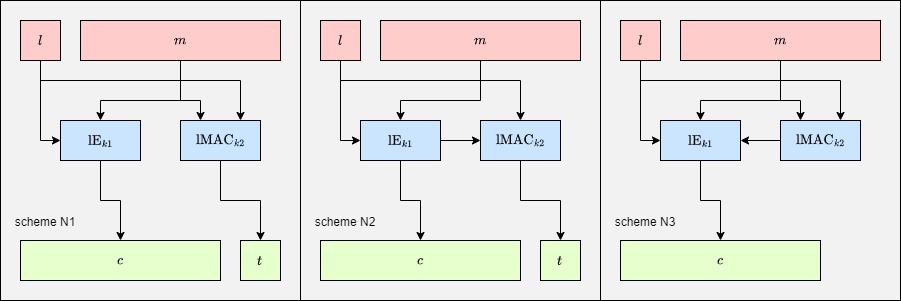
\includegraphics[scale = 0.4]{images/N-schemes.png}
\caption{Adjusted N schemes from \nrs}
\label{fig: N schemes}
\end{figure}

\begin{figure}
    \begin{pchstack}[boxed,center,space=0.5cm]
        \pseudocode[lnstart=-1,linenumbering,head={AE.enc$(\keyinstance,\lockinstance,\messageinstance)$}]{
            (\keyinstance{}1,\keyinstance{}2) \result \keyinstance \\
            \ciphertextinstance' \result \text{E.enc}(\keyinstance{}1,\lockinstance,\messageinstance) \\
            \taginstance \result \text{M.mac}(\keyinstance{}2,\lockinstance,\messageinstance) \\
            \ciphertextinstance \result (\ciphertextinstance',\taginstance)\\
            \pcreturn \ciphertextinstance
        }
        \pseudocode[lnstart=4,linenumbering,head={AE.dec$(\keyinstance,\lockinstance,\ciphertextinstance)$}]{
            (\keyinstance{}1,\keyinstance{}2) \result \keyinstance \\
            (\ciphertextinstance',\taginstance) \result \ciphertextinstance \\
            \messageinstance \result \text{E.dec}(\keyinstance{}1,\lockinstance,\ciphertextinstance') \\
            \taginstance' \result \text{M.mac}(\keyinstance{}2,\lockinstance,\messageinstance) \\
            \pcif \taginstance \neq \taginstance' : \messageinstance \result \invalid\\
            \pcreturn \messageinstance
        }
    \end{pchstack}
\caption{Calls based on N1}
\label{fig: N1 calls}
\end{figure}

\begin{figure}
    \begin{pchstack}[boxed,center,space=0.5cm]
        \pseudocode[lnstart=-1,linenumbering,head={AE.enc$(\keyinstance,\lockinstance,\messageinstance)$}]{
            (\keyinstance{}1,\keyinstance{}2) \result \keyinstance\\
            \ciphertextinstance' \result \text{E.enc}(\keyinstance{}1,\lockinstance,\messageinstance)\\
            \taginstance \result \text{M.mac}(\keyinstance{}2,\lockinstance,\ciphertextinstance')\\
            \ciphertextinstance \result (\ciphertextinstance',\taginstance)\\
            \pcreturn \ciphertextinstance
        }
        \pseudocode[lnstart=4,linenumbering,head={AE.dec$(\keyinstance,\lockinstance,\ciphertextinstance)$}]{
            (\keyinstance{}1,\keyinstance{}2) \result \keyinstance\\
            (\ciphertextinstance',\taginstance) \result \ciphertextinstance\\
            \messageinstance \result \text{E.dec}(\keyinstance{}1,\lockinstance,\ciphertextinstance')\\
            \taginstance' \result \text{M.mac}(\keyinstance{}2,\lockinstance,\ciphertextinstance')\\
            \pcif \taginstance \neq \taginstance' : \messageinstance \result \invalid\\
            \pcreturn \messageinstance
        }
    \end{pchstack}
\caption{Calls based on N2}
\label{fig: N2 calls}
\end{figure}

\begin{figure}
    \begin{pchstack}[boxed,center,space=0.5cm]
        \pseudocode[lnstart=-1,linenumbering,head={AE.enc$(\keyinstance,\lockinstance,\messageinstance)$}]{
            (\keyinstance{}1,\keyinstance{}2) \result \keyinstance\\
            \taginstance \result \text{M.mac}(\keyinstance{}2,\lockinstance,\messageinstance)\\
            \messageinstance' \result \messageinstance \concatinate \taginstance\\
            \ciphertextinstance \result E.enc(\keyinstance{}1,\lockinstance,\messageinstance')\\
            \pcreturn \ciphertextinstance
        }
        \pseudocode[lnstart=4,linenumbering,head={AE.dec$(\keyinstance,\lockinstance,\ciphertextinstance)$}]{
            (\keyinstance{}1,\keyinstance{}2) \result \keyinstance\\
            \messageinstance' \result \text{E.dec}(\keyinstance{}1,\lockinstance,\ciphertextinstance)\\
            (\messageinstance,\taginstance) \result \messageinstance'\\
            \taginstance' \result \text{M.mac}(\keyinstance{}2,\lockinstance,\messageinstance)\\
            \pcif \taginstance \neq \taginstance' : \messageinstance \result \invalid\\
            \pcreturn \messageinstance
        }
    \end{pchstack}
\caption{Calls based on N3}
\label{fig: N3 calls}
\end{figure}

\subsection{Security Bounds}
We define the constructions secure if there is a tight (\textbf{todo: look at tight sec reductions}) reduction from breaking the loAE-security of the scheme to breaking the loE-security or the loMAC security of the underlying primitives.
(\textbf{Note: This section is likely to contain some mistakes. I started trying to proof N2 as you said this would most likely be the easiest one. I plan to do N1 and N3 if you think the proof for N2 is correct.})

\newpage
\paragraph{N2}
first, we define our theorem:
\begin{theorem}
Let loAE be constructed from loMAC and loE as described in figure \ref{fig: N2 calls}. Then for any number of users \users{} and any loAE adversary \adversary{} that poses at most $Q_e$ many Oenc queries, limited by N, and at most $Q_d$ many Odec queries, there exist a loMAC adversary $B$ and a loE adversary $C$ such that:
\begin{align*}
    \text{\advantage{$A$,\users}{loAE}} = \text{\advantage{$B$,\users}{loMAC}} + \frac{Q_d}{\abs{t}^2} + \text{\advantage{$C$,\users}{loE}},
\end{align*}
where $\abs{t}$ is the output length of the loMAC. The running time of $B$ is at most that of A plus the time require to run $Q_e$ many E.enc encapsulations and $Q_d$ many E.dec decapsulations. The running time of $C$ is at most that of \adversary. Additionally, $B$ makes at most $Q_e$ many Omac queries and at most $Q_d$ many Ovrf queries and $C$ makes at most $Q_e$ many Oenc queries.
\end{theorem}
Within this theorem, both $Q_e$ and $Q_d$ refer to the total queries the adversary is allowed to make, not the queries per user. To prove this theorem we start by defining game loAE-N2 in figure \ref{fig: loAE-N2 game}. This game is the game loAE-IND-\$-CCA (figure \ref{fig: loAE-IND game}) AE.enc and AE.dec substituted with the N2 algorithms from figure \ref{fig: N2 calls}.
\begin{figure}[H]
    \begin{pchstack}[boxed,center,space=0.5cm]
        \pseudocode[lnstart=-1,linenumbering,head={\textbf{Game} loAE-N2$^{b}_{\adversary,\users}$ }]{
        L \result \emptyset\\
        \pcfor \user \in [1..N]:\\
        \t \keyinstance_\user \sample \keyspace\\
        \t C_\user \result \invalid\\
        b' \result \adversary\\
        \pcreturn b'
        }
        \pseudocode[lnstart=5,linenumbering,head={\textbf{Oracle} Oenc$(\user,\lockinstance,\messageinstance)$}]{
            \pcif C_\user \neq \invalid: \pcreturn \invalid\\
            \pcif \lockinstance \in L: \pcreturn \invalid\\
            L \result L \cup \{\lockinstance\}\\
            \lockinstance_\user \result \lockinstance\\
            (\keyinstance{}1,\keyinstance{}2) \result \keyinstance_j\\
            \ciphertextinstance' \result \text{E.enc}(\keyinstance{}1,\lockinstance_j,\messageinstance)\\
            \taginstance \result \text{M.mac}(\keyinstance{}2,\lockinstance_j,\ciphertextinstance')\\
            \ciphertextinstance \result (\ciphertextinstance',\taginstance)\\
            \pcif b = 1 \wedge \ciphertextinstance \neq \invalid: \\
            \t \ciphertextinstance \sample \{0,1\}^{\abs{\ciphertextinstance}}\\
            C_\user \result \ciphertextinstance\\
            \pcreturn \ciphertextinstance
        }
        \pseudocode[lnstart=17,linenumbering,head={\textbf{Oracle} Odec$(\user,\ciphertextinstance)$}]{
            \pcif C_\user = \invalid: \pcreturn \invalid\\
            \pcif \ciphertextinstance = C_\user: \pcreturn \invalid\\
            (\keyinstance{}1,\keyinstance{}2) \result \keyinstance_j\\
            (\ciphertextinstance',\taginstance) \result \ciphertextinstance\\
            \messageinstance \result \text{E.dec}(\keyinstance{}1,\lockinstance_j,\ciphertextinstance')\\
            \taginstance' \result \text{M.mac}(\keyinstance{}2,\lockinstance_j,\ciphertextinstance')\\
            \pcif \taginstance \neq \taginstance' : \messageinstance \result \invalid\\
            \pcif b = 1 : \messageinstance \result \invalid\\
            \pcreturn \messageinstance
        }
    \end{pchstack}
    \caption{loAE-N2 game, adversary{} has access to oracles Oenc and Odec.}
    \label{fig: loAE-N2 game}
\end{figure}

\noindent This gives us
\begin{align*}
    \text{\advantage{$A$,\users}{loAE}}
    =
    \text{Pr}[\text{loAE-N2}_{\text{\adversary,\users}}^0 =0]
    -
    \text{Pr}[\text{loAE-N2}_{\text{\adversary,\users}}^1 =0]
\end{align*}
Next we define game N2-switch-1 in figure \ref{fig: N2-switch-1 game}. The only difference between this game and game loAE-N2 is the fact that N2-switch-1 uses the uniformly random function $tag$, instead of the loMAC. This function takes the same input as the MAC would take, and outputs a uniformly random tag with the same length as the output tag from the MAC would have had.

\begin{figure}[H]
    \begin{pchstack}[boxed,center,space=0.5cm]
        \pseudocode[lnstart=-1,linenumbering,head={\textbf{Game} N2-switch-2$^{b}_{\adversary,\users}$ }]{
        L \result \emptyset\\
        \pcfor \user \in [1..N]:\\
        \t \keyinstance_\user \sample \keyspace\\
        \t C_\user \result \invalid\\
        b' \result \adversary\\
        \pcreturn b'
        }
        \pseudocode[lnstart=5,linenumbering,head={\textbf{Oracle} Oenc$(\user,\lockinstance,\messageinstance)$}]{
            \pcif C_\user \neq \invalid: \pcreturn \invalid\\
            \pcif \lockinstance \in L: \pcreturn \invalid\\
            L \result L \cup \{\lockinstance\}\\
            \lockinstance_\user \result \lockinstance\\
            (\keyinstance{}1,\keyinstance{}2) \result \keyinstance_j\\
            \ciphertextinstance' \result \text{E.enc}(\keyinstance{}1,\lockinstance_j,\messageinstance)\\
            \taginstance \result tag(\keyinstance{}2,\lockinstance_j,\ciphertextinstance')\\
            \ciphertextinstance \result (\ciphertextinstance',\taginstance)\\
            \pcif b = 1 \wedge \ciphertextinstance \neq \invalid: \\
            \t \ciphertextinstance \sample \{0,1\}^{\abs{\ciphertextinstance}}\\
            C_\user \result \ciphertextinstance\\
            \pcreturn \ciphertextinstance
        }
        \pseudocode[lnstart=17,linenumbering,head={\textbf{Oracle} Odec$(\user,\ciphertextinstance)$}]{
            \pcif C_\user = \invalid: \pcreturn \invalid\\
            \pcif \ciphertextinstance = C_\user: \pcreturn \invalid\\
            (\keyinstance{}1,\keyinstance{}2) \result \keyinstance_j\\
            (\ciphertextinstance',\taginstance) \result \ciphertextinstance\\
            \messageinstance \result \text{E.dec}(\keyinstance{}1,\lockinstance_j,\ciphertextinstance')\\
            \taginstance' \result tag(\keyinstance{}2,\lockinstance_j,\ciphertextinstance')\\
            \pcif \taginstance \neq \taginstance' : \messageinstance \result \invalid\\
            \pcif b = 1 : \messageinstance \result \invalid\\
            \pcreturn \messageinstance
        }
    \end{pchstack}
    \caption{N2-switch-1, adversary{} has access to oracles Oenc and Odec.}
    \label{fig: N2-switch-1 game}
\end{figure}

\noindent
Using this game, we expand the probability:
\begin{align*}
    \text{\advantage{$A$,\users}{loAE}}
    &=
    \text{Pr}[\text{loAE-N2}_{\text{\adversary,\users}}^0 =0]
    -
    \text{Pr}[\text{N2-switch-1}_{\text{\adversary,\users}}^0 =0]
    \\& \hspace{0,3cm}  + \text{Pr}[\text{N2-switch-1}_{\text{\adversary,\users}}^0 =0]
    -
    \text{Pr}[\text{loAE-N2}_{\text{\adversary,\users}}^1 =0]
\end{align*}
Any adversary \adversary{} winning game loAE-N2, but not N2-switch-1, can break the security of the loMAC. Concretely, we define adversary $B$ against loMAC that wins security game loMAC-PRF (figure \ref{fig: loMAC-PRF game}) using \adversary.
\begin{figure}[H]
    \begin{pchstack}[boxed,center,space=0.5cm]
        \pseudocode[lnstart=-1,linenumbering,head={\textbf{Adverary} $B$}]{
        L \result \emptyset\\
        \pcfor \user \in [1..N]:\\
        \t \keyinstance_\user \sample \keyspace\\
        \t C_\user \result \invalid\\
        b' \result \textbf{run } \adversary\\
        \pcreturn b'
        }
        \pseudocode[lnstart=5,linenumbering,head={\text{if \adversary{} calls }\textbf{Oracle} Oenc$(\user,\lockinstance,\messageinstance)$}]{
            \pcif C_\user \neq \invalid: \pcreturn \invalid\\
            \pcif \lockinstance \in L: \pcreturn \invalid\\
            L \result L \cup \{\lockinstance\}\\
            \lockinstance_\user \result \lockinstance\\
            \ciphertextinstance' \result \text{E.enc}(\keyinstance_j,\lockinstance_j,\messageinstance)\\
            \taginstance \result \text{Omac}(\user,\lockinstance_j,\ciphertextinstance')\\
            \ciphertextinstance \result (\ciphertextinstance',\taginstance)\\
            C_\user \result \ciphertextinstance\\
            \pcreturn \ciphertextinstance
        }
        \pseudocode[lnstart=14,linenumbering,head={\text{if \adversary{} calls }\textbf{Oracle} Odec$(\user,\ciphertextinstance)$}]{
            \pcif C_\user = \invalid: \pcreturn \invalid\\
            \pcif \ciphertextinstance = C_\user: \pcreturn \invalid\\
            (\ciphertextinstance',\taginstance) \result \ciphertextinstance\\
            \messageinstance \result \text{E.dec}(\keyinstance{}_j,\lockinstance_j,\ciphertextinstance')\\
            passed \result \text{Ovrf}(\user,\ciphertextinstance',\taginstance')\\
            \pcif \neg passed : \messageinstance \result \invalid\\
            \pcreturn \messageinstance
        }
    \end{pchstack}
    \caption{Adversary $B$, has access to \adversary{} and oracles Omac and Ovrf. Note that $\keyinstance_\user$ is the MAC key in this game.}
    \label{fig: adversary B N2}
\end{figure}


\noindent
This adversary has the runtime of \adversary{}. For every Oenc query \adversary{} makes, $B$ computes E.enc once, and call Omac once. For every Odec query \adversary{} makes, $B$ computes E.dec once and calls Ovrf once. Note that, alternatively, $B$ could return 0 if $passed$ is \codetrue{} to avoid having to do E.dec computations. To increase consistency with the other two cases, these computations are still made. Using $B$, we can see that $\text{Pr}[\text{loMAC-PRF}_{\text{\adversary,\users}}^0 =0]=\text{Pr}[\text{loAE-N2}_{\text{\adversary,\users}}^0 =0]$ as $B$ simulates game loAE-N2 with $b$ = 0 whenever its own $b$ is 0. In addition, we can see that $\text{Pr}[\text{loMAC-PFR}_{\text{\adversary,\users}}^1 =0]=\text{Pr}[\text{N2-switch-1}_{\text{\adversary,\users}}^0 =0]$ as $B$ simulates game N2-switch-1 with $b$ = 0 whenever its own $b$ is 1. As a result we can rewrite our probability to:
\begin{align*}
    \text{\advantage{$A$,\users}{loAE}}
    &=
    \text{Pr}[\text{loAE-N2}_{\text{\adversary,\users}}^0 =0]
    -
    \text{Pr}[\text{N2-switch-1}_{\text{\adversary,\users}}^0 =0]
    \\& \hspace{0,3cm} + \text{Pr}[\text{N2-switch-1}_{\text{\adversary,\users}}^0 =0]
    -
    \text{Pr}[\text{loAE-N2}_{\text{\adversary,\users}}^1 =0]
    \\& =
    \text{Pr}[\text{loMAC-PRF}_{\text{\adversary,\users}}^0 =0]
    -
    \text{Pr}[\text{loMAC-PRF}_{\text{\adversary,\users}}^1 =0]
    \\& \hspace{0,3cm} + \text{Pr}[\text{N2-switch-1}_{\text{\adversary,\users}}^0 =0]
    -
    \text{Pr}[\text{loAE-N2}_{\text{\adversary,\users}}^1 =0]
    \\& = \text{\advantage{$B$,\users}{loMAC}}
    + \text{Pr}[\text{N2-switch-1}_{\text{\adversary,\users}}^0 =0]
    -
    \text{Pr}[\text{loAE-N2}_{\text{\adversary,\users}}^1 =0]
\end{align*}
To expand our probability again, we define game N2-switch-2 in figure \ref{fig: N2-switch-2 game}. The only difference between this game and the first switch game is that game 2 will always return \invalid{} when the Odec query is called. We use this game to expand our probability twice:
\begin{align*}
    \text{\advantage{$A$,\users}{loAE}}
    &\leq
    \text{\advantage{$B$,\users}{loMAC}} 
    +
    \text{Pr}[\text{N2-switch-1}_{\text{\adversary,\users}}^0 =0]
    -
    \text{Pr}[\text{N2-switch-2}_{\text{\adversary,\users}}^0 =0]
    \\& \hspace{0,3cm}+
    \text{Pr}[\text{N2-switch-2}_{\text{\adversary,\users}}^0 =0]
    -
    \text{Pr}[\text{N2-switch-2}_{\text{\adversary,\users}}^1 =0]
    \\& \hspace{0,3cm}+
    \text{Pr}[\text{N2-switch-2}_{\text{\adversary,\users}}^1 =0]
    -
    \text{Pr}[\text{loAE-N2}_{\text{\adversary,\users}}^1 =0]
\end{align*}
\begin{figure}[H]
    \begin{pchstack}[boxed,center,space=0.5cm]
        \pseudocode[lnstart=-1,linenumbering,head={\textbf{Game} N2-switch-2$^{b}_{\adversary,\users}$ }]{
        L \result \emptyset\\
        \pcfor \user \in [1..N]:\\
        \t \keyinstance_\user \sample \keyspace\\
        \t C_\user \result \invalid\\
        b' \result \adversary\\
        \pcreturn b'
        }
        \pseudocode[lnstart=5,linenumbering,head={\textbf{Oracle} Oenc$(\user,\lockinstance,\messageinstance)$}]{
            \pcif C_\user \neq \invalid: \pcreturn \invalid\\
            \pcif \lockinstance \in L: \pcreturn \invalid\\
            L \result L \cup \{\lockinstance\}\\
            \lockinstance_\user \result \lockinstance\\
            (\keyinstance{}1,\keyinstance{}2) \result \keyinstance_j\\
            \ciphertextinstance' \result \text{E.enc}(\keyinstance{}1,\lockinstance_j,\messageinstance)\\
            \taginstance \result tag(\keyinstance{}2,\lockinstance_j,\ciphertextinstance')\\
            \ciphertextinstance \result (\ciphertextinstance',\taginstance)\\
            \pcif b = 1 \wedge \ciphertextinstance \neq \invalid: \\
            \t \ciphertextinstance \sample \{0,1\}^{\abs{\ciphertextinstance}}\\
            C_\user \result \ciphertextinstance\\
            \pcreturn \ciphertextinstance
        }
        \pseudocode[lnstart=17,linenumbering,head={\textbf{Oracle} Odec$(\user,\ciphertextinstance)$}]{
            \pcreturn \invalid
        }
    \end{pchstack}
    \caption{N2-switch-2 game, adversary{} has access to oracles Oenc and Odec.}
    \label{fig: N2-switch-2 game}
\end{figure}

\noindent
In the real world, the oracle Odec from N2-switch-1 returns \invalid{}, unless the condition on line 24 is false. As a result, $\text{Pr}[\text{N2-switch-1}_{\text{\adversary,\users}}^0 =0] - \text{Pr}[\text{N2-switch-2}_{\text{\adversary,\users}}^0 =0]$ will be equal to the chance of this condition being true. As \taginstance{} and \taginstance' are the result of the uniformly random function $tag$, where the input of $tag$ may not be equal when computing both, the chance of \taginstance{} and \taginstance' being equal will be $\frac{1}{\abs{t}^2}$ for every Odec calls. Combining this with at most $Q_d$ calls to the decryption oracle, we get:
\begin{align*}
    \text{\advantage{$A$,\users}{loAE}}
    &\leq
    \text{\advantage{$B$,\users}{loMAC}} 
    + \frac{Q_d}{\abs{t}^2} +
    \text{Pr}[\text{N2-switch-2}_{\text{\adversary,\users}}^0 =0]
    -
    \text{Pr}[\text{N2-switch-2}_{\text{\adversary,\users}}^1 =0]
    \\& \hspace{0,3cm}+
    \text{Pr}[\text{N2-switch-2}_{\text{\adversary,\users}}^1 =0]
    -
    \text{Pr}[\text{loAE-N2}_{\text{\adversary,\users}}^1 =0]
\end{align*}
In N2-switch-2, no information can ever be gained from making a Odec query. As a result any adversary $A$ winning this game can break break the security of the loE as well. Concretely, we define adversary $C$ against loE that wins game loE-IND-\$-CPA using this \adversary. Adversary $C$ forwards all Oenc queries and disregards all Odec queries. The runtime of $C$ is that of $A$ and $C$ makes $Q_e$ many Oenc queries. This leads to:
\begin{align*}
    \text{Pr}[\text{N2-switch-2}_{\text{$C$,\users}}^0 =0] - \text{Pr}[\text{N2-switch-2}_{\text{$C$,\users}}^1 =0]& = \text{\advantage{$C$,\users}{loE}}
\end{align*}
In addition to this, games N2-switch-2 and loAE-N2 are equal in the ideal world, resulting in $\text{Pr}[\text{N2-switch-2}_{\text{\adversary,\users}}^1 =0]
-
\text{Pr}[\text{loAE-N2}_{\text{\adversary,\users}}^1 =0]$ = 0. Filling both these in gives us our final result:
\begin{align*}
    \text{\advantage{$A$,\users}{loAE}}
    &\leq
    \text{\advantage{$B$,\users}{loMAC}} 
    + \frac{Q_d}{\abs{t}^2} +
    \text{\advantage{$C$,\users}{loE}}
\end{align*}

\subsection{Comparison with Existing Alternatives}

\section{Use Cases}
should consist of:
\begin{itemize}
	\item possible use cases
\end{itemize}
\subsection{PKE Schemes}

\section{Related Work}
\textbf{Location not final yet}

\section{Conclusion}

\newpage
\printbibliography[heading=bibintoc,title={References}]
\section*{Appendix A}
(\textbf{todo: elaborate more on this table})\\
Below is a table which highlights the differences in notation between \gkp{} and \nrs, as well as give the notation I will be using.\\
\begin{tabular}[H]{|c | c | c | c | m{4,5cm}|}
    \hline
    Name   &   \gkp   &   \nrs   &   my notation & rough meaning \\[0.5 ex]
    \hline
    \hline
    message   &   $m$   &   $M$   &   \messageinstance &  message the user sends \\
    \hline
    ciphertext space   &   $\mathcal{C}$   &   -   &   \ciphertextspace & set of all possible ciphertext options \\
    \hline
    ciphertext   &   $c$   &   $C$   &   \ciphertextinstance & encrypted message \\
    \hline
    associated data   &   -   &   $A$   &   \associateddatainstance & data you want to authenticate but not encrypt \\
    \hline
    tag space   &   $\mathcal{C}$   &   -   &   \tagspace & set off all possible tag options \\
    \hline
    tag   &   $c$   &   $T$   &   \taginstance & output of MAC function \\
    \hline
    key   &   $k$   &   $K$   &   \keyinstance   & user key \\
    \hline
    nonce space   &   -   &   $\mathcal{N}$   &   \noncespace & set of all nonce options \\
    \hline
    nonce   &   -   &   $n$   &   \nonceinstance & number only used once \\
    \hline
    lock space   &   $\mathcal{T}$   &   -   &   \lockspace & set of all possible lock options \\
    \hline
    lock   &   $t$   &   -   &   \lockinstance & nonce that is bound to the user \\
    \hline
    adversary   &   A   &   $\mathcal{A}$   &   \adversary & the bad guy \\
    \hline
    random sampling   &   $\xleftarrow{\$}$    &   $\twoheadleftarrow$   &   \sample & get a random ellement from the set \\
    \hline
    result of randomized function   &   $\xleftarrow{\$}$   &   -   &   \result & get the result of a randomized function with given inputs \\
    \hline
    %Name   &   \gkp   &   \GCrec   &   my notation & rough meaning \\
    %\hline
\end{tabular}

\end{document}

\NeedsTeXFormat{LaTeX2e}
\ProvidesPackage{rutitlepage}[2022/02/21 Mart Lubbers]
\RequirePackage{geometry,graphicx,ifpdf,keyval,iflang}
\def\@rutitleauthors{\@author}
\def\@rutitleauthorstext{Aut\IfLanguageName{dutch}{eu}{ho}r:}
\def\@rutitledate{\@date}
\def\@rutitleinst{Radboud Universit\IfLanguageName{dutch}{eit}{y} Nijmegen}
\def\@rutitletitle{\@title}
\def\@rutitlelayout{twentytwo}
\newif\if@rutitlecolour\@rutitlecolourfalse
\define@key{maketitleru}{authors}{\def\@rutitleauthors{#1}}
\define@key{maketitleru}{authorstext}{\def\@rutitleauthorstext{#1}}
\define@key{maketitleru}{colour}[true]{\@rutitlecolourtrue}
\define@key{maketitleru}{course}{\def\@rutitlecourse{#1}}
\define@key{maketitleru}{date}{\def\@rutitledate{#1}}
\define@key{maketitleru}{institution}{\def\@rutitleinst{#1}}
\define@key{maketitleru}{layout}{\def\@rutitlelayout{#1}}
\define@key{maketitleru}{nextpagenr}{\def\@rutitlenextpagenr{#1}}
\define@key{maketitleru}{others}{\def\@rutitleothers{#1}}
\define@key{maketitleru}{subtitle}{\def\@rutitlesubtitle{#1}}
\define@key{maketitleru}{title}{\def\@rutitletitle{#1}}
\newcommand*{\rutitlepage@printothers}[2]{\textit{#1}\\#2}
\newcommand*{\rutitlepage@sepothers}{\\[\baselineskip]}
\newcommand*{\rutitlepage@others}[2]{%
	\rutitlepage@printothers{#1}{#2}%
	\kernel@ifnextchar,{\rutitlepage@sepothers\rutitlepage@otherslist@}\relax}
\newcommand*{\rutitlepage@otherslist}[1]{%
	\expandafter\rutitlepage@others#1}
\def\rutitlepage@otherslist@,#1{\rutitlepage@otherslist{{#1}}}
\newcommand{\rutitle@layout@twentytwo}[0]{
	\newgeometry{left=25mm,top=25mm,right=15mm,bottom=10mm,hmarginratio=1:1}
	\begin{titlepage}%
		\null\vfill%
		\parindent0pt
		\ifdefined\@rutitlecourse\textsc{\LARGE\@rutitlecourse}\\[1.5cm]\fi
		{\Huge\bfseries\@rutitletitle}%
		\ifdefined\@rutitlesubtitle{\\[2\baselineskip]\large\itshape\@rutitlesubtitle\/}\fi\\[4\baselineskip]
		{\Large\scshape\@rutitleauthors}\\[\baselineskip]
		{\large\@rutitledate}
		\vfill

		\ifdefined\@rutitleothers\rutitlepage@otherslist\@rutitleothers\fi
		\vfill

		\hfill
		\ifpdf\includegraphics[width=80mm]{rutitlepage-logo-\IfLanguageName{dutch}{nl-}{}\if@rutitlecolour cmyk\else bw\fi.pdf}\\
		\else\includegraphics[width=80mm]{rutitlepage-logo-\IfLanguageName{dutch}{nl-}{}\if@rutitlecolour cmyk\else bw\fi.eps}\\
		\fi
	\end{titlepage}
	\restoregeometry%
}
\newcommand{\rutitle@layout@seventeen}[0]{
	\newgeometry{left=25mm,top=25mm,right=15mm,bottom=10mm,hmarginratio=1:1}
	\begin{titlepage}%
		\null\vfill%
		\parindent0pt
		{\Huge\bfseries\@rutitletitle}%
		\ifdefined\@rutitlesubtitle{\\[2\baselineskip]\large\itshape\@rutitlesubtitle\/}\fi\\[4\baselineskip]
		{\Large\scshape\@rutitleauthors}\\[\baselineskip]
		{\large\@rutitledate}
		\vfill

		\ifdefined\@rutitleothers\rutitlepage@otherslist\@rutitleothers\fi
		\vfill

		\hfill
		\ifpdf\includegraphics[width=80mm]{rutitlepage-logo-\IfLanguageName{dutch}{nl-}{}\if@rutitlecolour cmyk\else bw\fi.pdf}\\
		\else\includegraphics[width=80mm]{rutitlepage-logo-\IfLanguageName{dutch}{nl-}{}\if@rutitlecolour cmyk\else bw\fi.eps}\\
		\fi
	\end{titlepage}
	\restoregeometry%
}
\newcommand{\rutitle@layout@traditional}[0]{
	\newgeometry{hmarginratio=1:1}
	\begin{titlepage}
		\begin{center}
			\ifdefined\@rutitlecourse\textsc{\LARGE\@rutitlecourse}\\[1.5cm]\fi
			\ifpdf\includegraphics[height=150pt]{rutitlepage-logo.pdf}\\
			\else\includegraphics[height=150pt]{rutitlepage-logo.eps}\\
			\fi
			\vspace{0.4cm}
			\textsc{\Large\@rutitleinst}\\[1cm]
			\hrule
			\vspace{0.4cm}
			\textbf{\large\@rutitletitle}\\[0.4cm]
			\hrule
			\ifdefined\@rutitlesubtitle
				\vspace{0.4cm}
				\textit{\@rutitlesubtitle}\\[1cm]
			\else
				\vspace{2cm}
			\fi
			\begin{minipage}[t]{0.45\textwidth}
				\begin{flushleft}\large
					\textit{\@rutitleauthorstext}\\
					\@rutitleauthors{}
				\end{flushleft}
			\end{minipage}
			\begin{minipage}[t]{0.45\textwidth}
				\begin{flushright}\large
					\ifdefined\@rutitleothers
					\renewcommand{\rutitlepage@printothers}[2]{\textit{##1}\\##2}
					\renewcommand{\rutitlepage@sepothers}[0]{

						\vspace{8mm}}
					\rutitlepage@otherslist\@rutitleothers
					\fi
				\end{flushright}
			\end{minipage}
			\vfill
			{\large\@rutitledate}
		\end{center}
	\end{titlepage}
	\restoregeometry%
}
\newcommand{\maketitleru}[1][]{
	\setkeys{maketitleru}{#1}
	\ifcsname%
		rutitle@layout@\@rutitlelayout\endcsname
		\expandafter\csname rutitle@layout@\@rutitlelayout\endcsname
	\else
		\PackageError{rutitlepage}
			{Unknown layout `\@rutitlelayout'.}
			{The `layout' key of \maketitleru\space contained an unknown layout.\MessageBreak{}
			 Check the package documentation for the possible layouts.}
	\fi
	\ifdefined\@rutitlenextpagenr\setcounter{page}{\@rutitlenextpagenr}\fi%
}